\chapter{Common Analysis Items}
\label{chapter:common_analysis_items}

\epigraph{\textit{First, you crack an egg into a small bowl.}}{--Unnamed Cookbook}

%todo fill in the citations
After the collisions and interactions in the LHC, final state particles leave their mark on various detector components as electronic signals. These electronic signals are saved in hard disks and tapes. It takes various steps of reconstruction identification, cleaning and calibration before the raw electronic information becomes analysis-ready physics objects. The different interactions particles have on various detector components create different distinct signatures for their identifications.
Figure~\ref{fig:particleSignature} shows the different signatures that different particles leave on the ATLAS detector.

In this chapter, various analysis final state objects are described. In Section~\ref{sec:Tracks}, detector tracks and vertex construction is covered. In Section~\ref{sec:Muon}, Section~\ref{sec:Jet} and Section~\ref{sec:Photon}, the formation of muons, jets and photons from detector signal
through their reconstruction, identification, isolation as well as calibration are discussed in detail. 

\begin{figure}[!htb]
    \begin{center}
        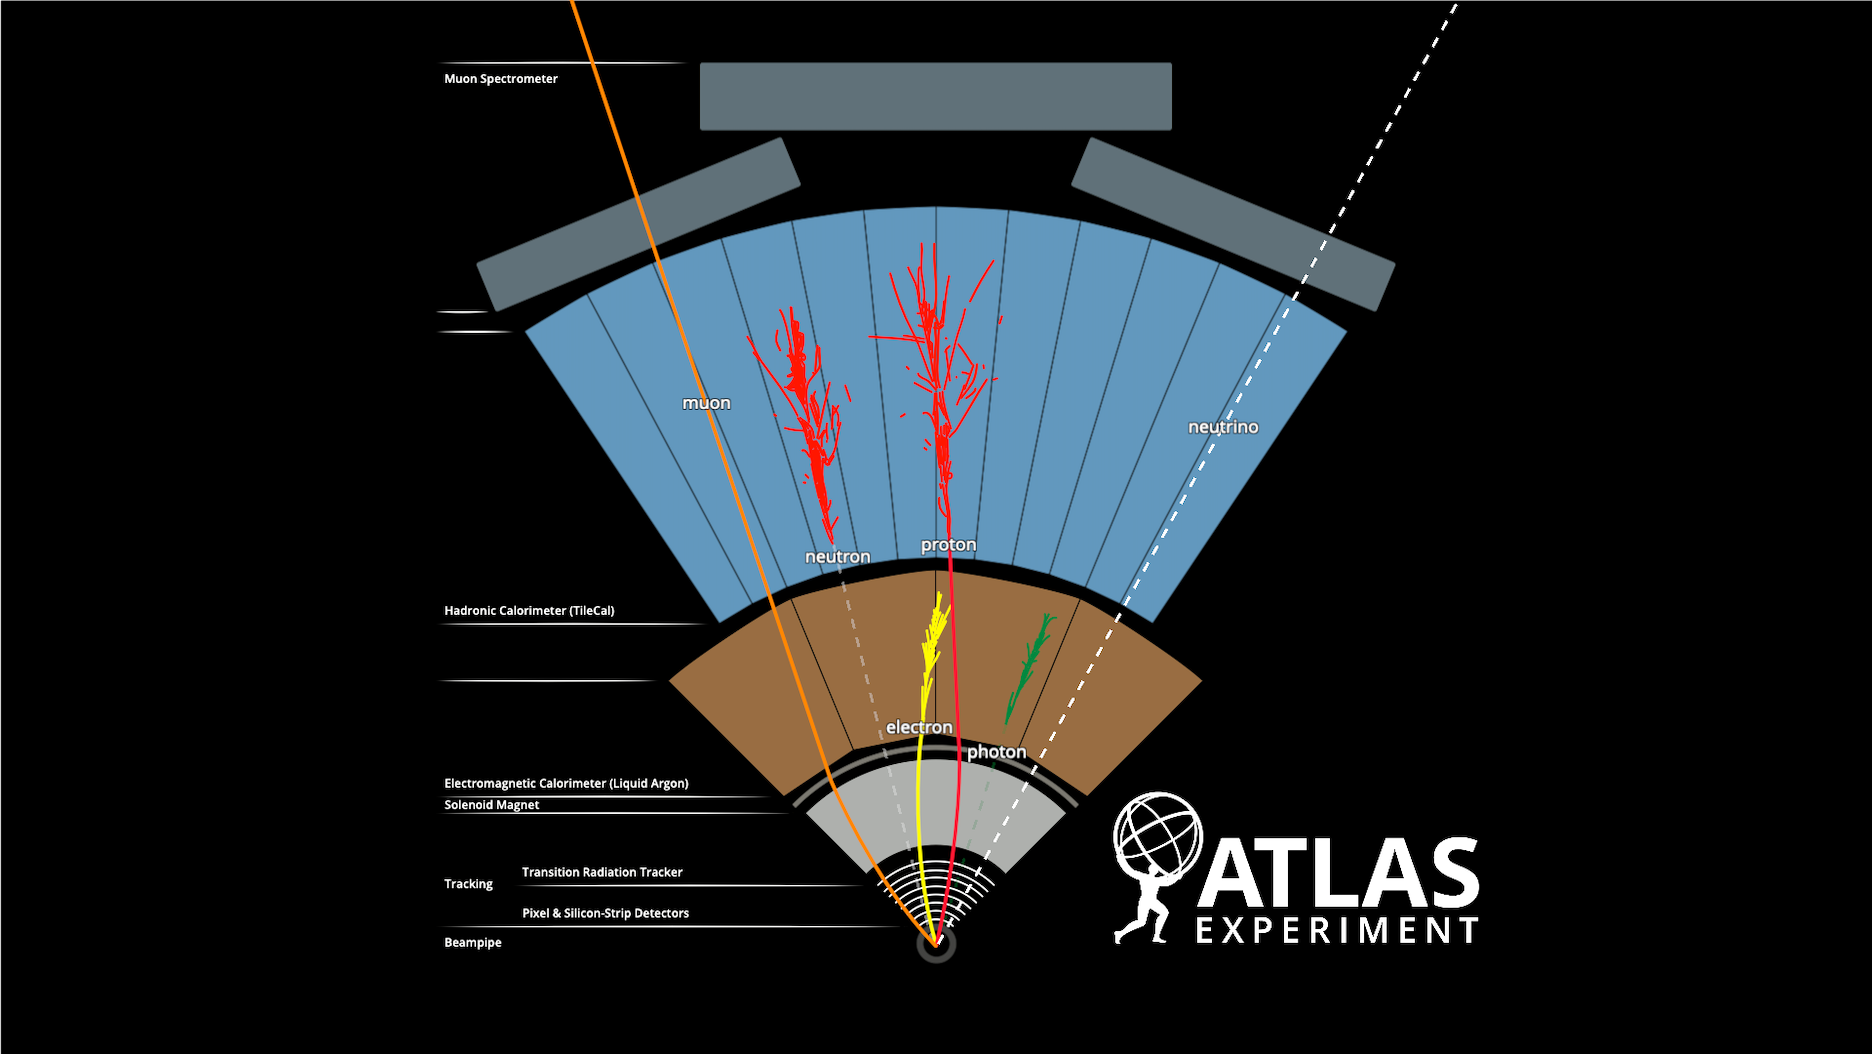
\includegraphics[width=1.1\textwidth]{figures/common_ana/ParticleSignature}
        \caption{        
            Particles displays distinct signatures~\cite{Mehlhase:2770815}.
        }
        \label{fig:particleSignature}
    \end{center}
\end{figure}

\section{Tracks and vertices}
\label{sec:Tracks}
Charged particles leave trajectories in two distinct ATLAS sub-detector systems, namely the inner detector(ID) and some also reach the the muon system(MS). Details regarding the subdetector system can be found in Chapter~\ref{chapter:ATLAS}.

\subsection{ID Tracks}
Hits is registered in an active detector element when a particle deposited enough energy to reach a predefined signal-to-noise(S/N) ratio. To reconstruct a track from detector raw hit information, coincidence measurements in multiple layers are first used to find a track seed. Then, a Kalman-filter is used to fit the tracks~\cite{track}, irrelevant hits from pileup~\footnote{Pileups are hits and tracks that result from multiple collisions other than the primary collision. In-time pileups are hit and tracks that came from interactions during the same collision event, out-of-time pileups are hits and tracks
comes from collisions of different event.} are removed through the filter. Figure~\ref{fig:track} shows a schematic diagram for a track.

\begin{figure}[!htb]
    \begin{center}
        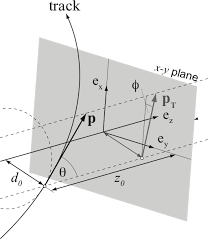
\includegraphics[width=0.3\textwidth]{figures/common_ana/Track}
        \caption{ 
        Schematic view of how the parameters associated with track creation in ATLAS.
        }
        \label{fig:track}
    \end{center}
\end{figure}

\subsection{Vertices}
Once tracks are formed in the inner detector, primary vertices can be constructed from the track directions and their intersection points. Vertexing picks out tracks and hits that are associated with a single interaction. It is helpful in discriminating event-of-interest tracks from pileup tracks. Effective vertexing is of great importance to event reconstruction, especially in more recent LHC runs, where the higher luminosity has resulted in additional in-time and out-of-time pileups.

\begin{figure}[!htb]
    \begin{center}
        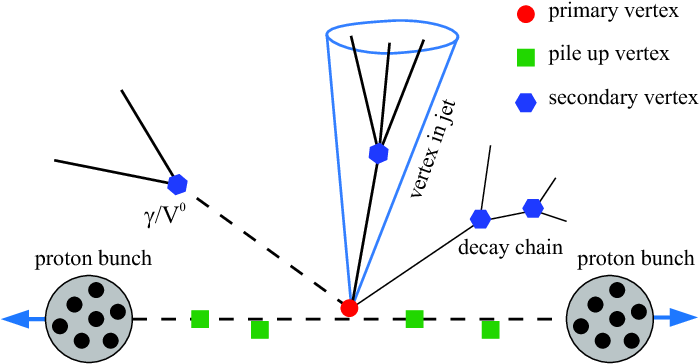
\includegraphics[width=0.4\textwidth]{figures/common_ana/Vertex}
        \caption{        
            Schematic view showing vertexing in ATLAS\cite{4774734}.
        }
    \end{center}
\end{figure}

Vertexing consists of a couple of different steps: First, a vertex seed is found by filtering the points where most interactions are found. Then, tracks consistent with the chosen vertex seed are put into a group. After that, the vertex position and the associated error of the vertex is found by an adaptive vertex fitting algorithm~\cite{track}. Lastly, the unused tracks are used for the next vertex creation. The process then repeats until no tracks remain. 

The vertex with the highest $P_{T}$ particles originated from it is considered the hard-primary vertex of the event, the others are considered the pileup primary vertices. Somtimes particles produced from the primary vertex decays further, the interaction points where the further decay occur are known as the secondary vertices.

Particle formation from detector hit information in the following sections relies on the tracks and primary vertex reconstruction above.

\section{Muons}
\label{sec:Muon}
Muons in ATLAS are formed from both the tracks and primary vertex information described in the above section. Muon reconstruction mainly relies on ID and MS information, while information from the calorimeter is sometimes also used for low $P_{T}$ muons. There are four different muon reconstruction strategies, as different transverse momentum($P_{T}$) ranges and detector hit locations leave distrinct muon signatures. From these four reconstruction strategies, four muon
working points, which are muons set in events chosen with pre-defined criteria, are derived~\cite{Aad:2746302}.

\begin{figure}[!htb]
    \begin{center}
        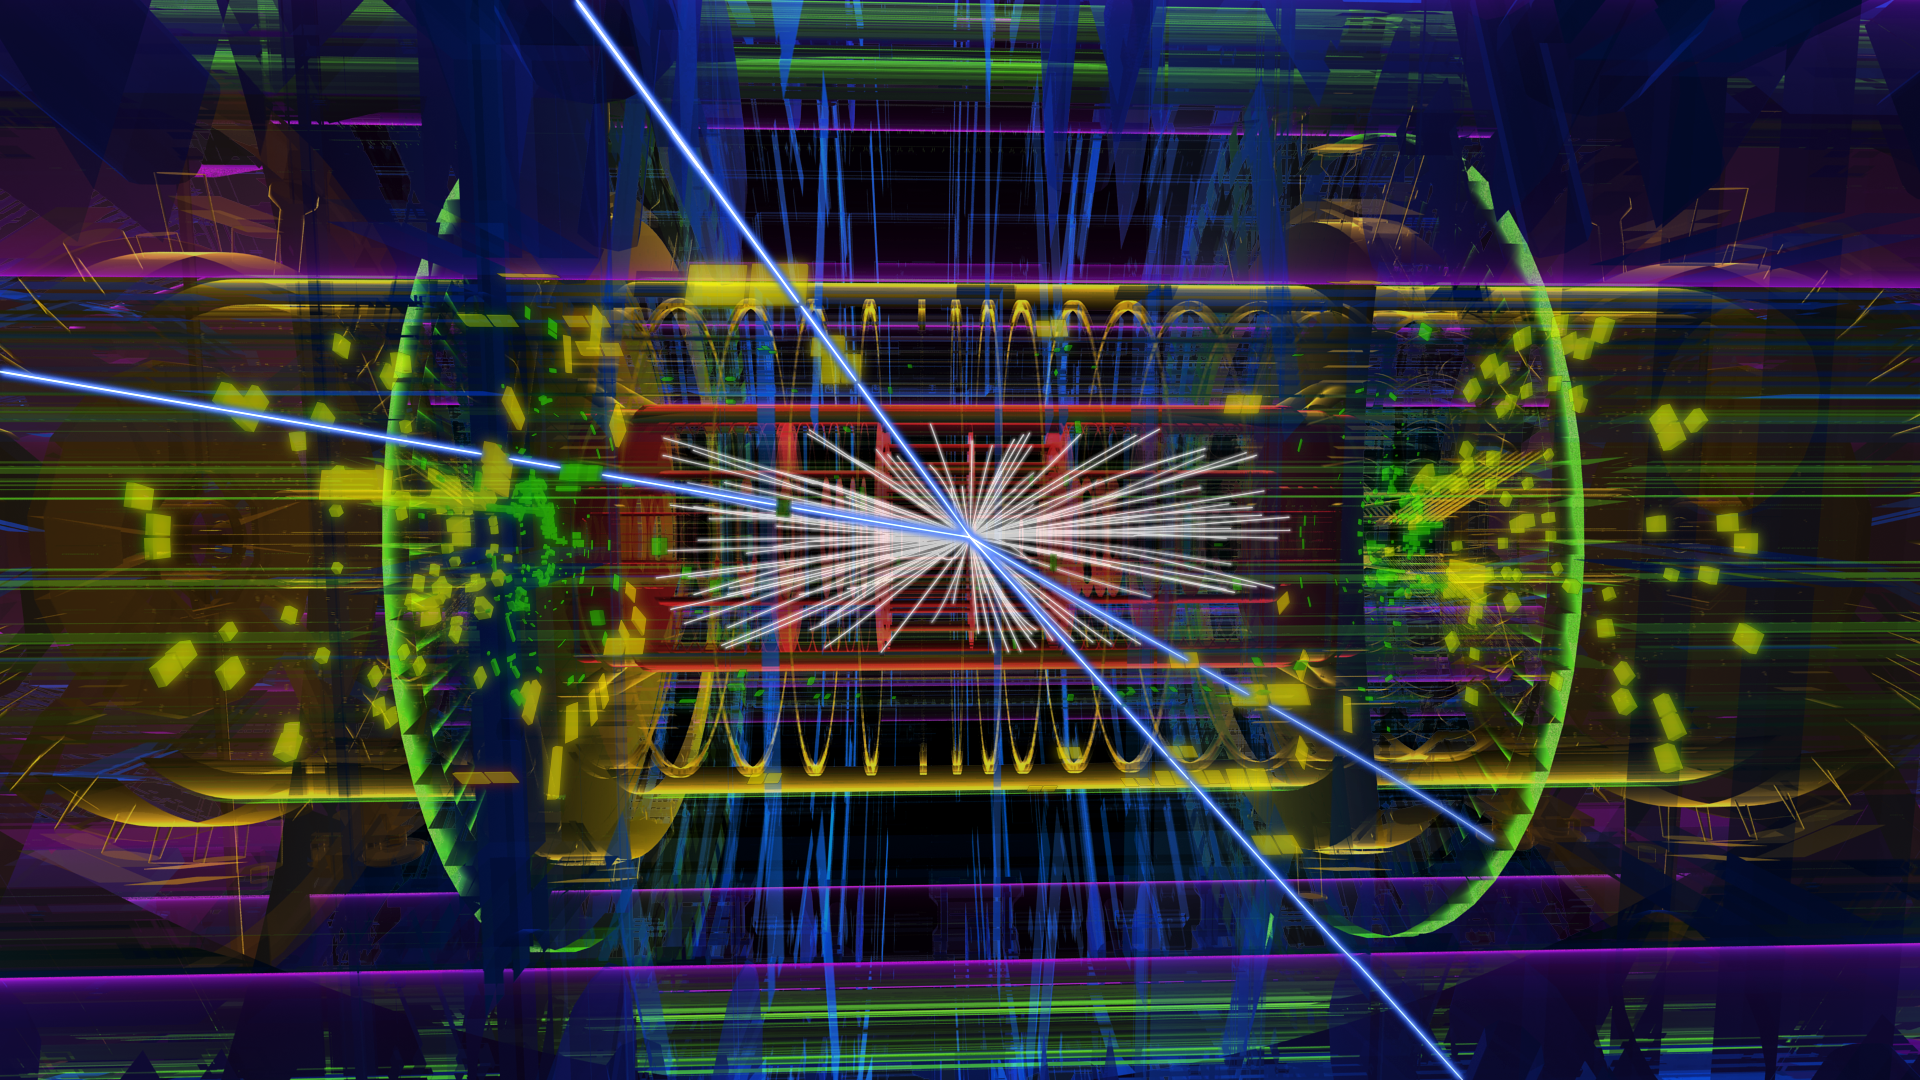
\includegraphics[width=0.5\textwidth]{figures/common_ana/Muon}
        \caption{        
            Visualization of a four muons event in the ATLAS detector\cite{ATLAS:1697053}. The four muons are visualized as blue tracks that travel from the primary interaction point through the inner dectector, the calorimeter and the muon system to beyond the detector.
        }
        \label{fig:muon}
    \end{center}
\end{figure}

\subsection{Muon Reconstruction}
Reconstruction of muons is performed in the following way: tracks are found in one part of the detector through pattern finding of hits in the ID/MS chambers. At least two matching segments from different subdetector parts are needed to form a track candidate. From the track candidate formed, global $\chi^{2}$ fits are performed, outliers from the fit is dropped and hits along the fitted track is added. Though they all share a common principle, various detailed reconstruction strategies are used for muons in
different $P_{T}$ ranges and detector locations to maximize reconstruction efficiencies~\cite{muonReco2016}.

\begin{itemize}
\item \textbf{Combined muon(CB)}
    This strategy is optimal for the muons that are detected in both the ID and the MS. It applies for muons found in both the barrel and end-cap region of the detector. Tracks are constructed from each of the ID and the MS. A global refit is done to remove outliers to improve the fit quality. This is first done by an outside-in approach where the tracks in MS are matched with tracks in the ID. Combined muons are also complemented by the inside-out muons: It looks for MS hits that can be associated with ID tracks and recovers muons that don't make it to the MS completely.

\item \textbf{Segment-tagged muons(ST)}
This method is used to identify lower $P_{T}$ muons that do not travel to the MS. If a track in the ID can be matched to at least one track segment in the MDT in the barrel or CSC in the end-cap, it will be selected as a segment-tagged muon. 

\item \textbf{Calorimeter-tagged muon(CT)}
    This reconstruction method is used for even lower $P_{T}$ muons that do not have enough energy reach the MS. Muons between 15 GeV $< P_{T} < $ 100GeV are formed from matching a track in ID with energy deposits in the calorimeter that match the minimum-ionizing particle. This is optimized for barrel muons of $|\eta| <0.1$. 

\item \textbf{Extrapolated muon(ME)}
    This reconstruction strategy is designed for muons that are very forward and are buried under noise from pileup. Muon tracks in the MS with a loose compatibility to the originating IP are accepted as ME muons. This strategy extends the acceptance of muons in the forward region from $2.5<|\eta|<2.7$. As there is no ID coverage in this region, other methods are not applicable.
\end{itemize}

\subsection{Muon Identification}
In ATLAS, the muon of interest are the muons that comes from the hard primary vertex decay. Muons formed this way are known as "prompt muons". "Non-Prompt" muons came from the semileptonic decay from jet fragmentations. Muon identification is a set of selection criteria applied to the candidate muons to cut out ``non-prompted" muons from light hadron decays that would result in in-flight detector production of muons. In different analyses, depending on the signal type, several muon identification working points are used.

A couple of criteria are used for muon identification: $q/p_{\textrm{significance}}$, $\rho'$ and $\chi^{2}_{\textrm{norm}}$. They are defined as ~\cite{muonReco2016}:

\subsubsection*{Discrimination Criteria}
\begin{itemize}

\item \textbf{q/p significance}
    \begin{equation}
    q/p_{\textrm{significance}} = |(q/p)^{ID} - (q/p)^{MS}|/\sqrt{\sigma^{MS}_{P_{T}} + \sigma^{ID}_{P_{T}}}
    \end{equation}

    This is the absolute value of the difference between the charges and the $P_{T}$ measurement divided by the sum of error in the $P_{T}$ measurement of both the ID and MS. $q$ is the charge, and p is the momentum of the particle. It is expected that the value is smaller for prompt muons as the particle will have similar $q/p$ ratio in both the ID and the MS if muon was created in the primary vertices rather than jet fragmentation later on. 

\item \textbf{$\rho'$}
    \begin{equation}
        \rho' = |P_{T}^{MS} - P_{T}^{ID}| / P_{T}^{\textrm{Combined}}
    \end{equation}

This is the absolute value of the difference between the $P_{T}$ of the MS and the ID divided by the combined $P_{T}$ of the muon candidate. A smaller value indicate a better match between the ID muon and the MS muon candidate.

\item \textbf{$\chi_{\textrm{norm}}^{2}$}

    This is the $\chi^{2}$ of the fit from the combined muon track from both the ID and MS. A smaller value shows that the ID and MS muon track candidates have the same direction and is therefore more likely to originate from a ``prompt muon".

\end{itemize}

These selection criteria for the muon groups above result in five different working points.

\subsubsection*{Muon Working Points}
\begin{itemize}

\item \textbf{MEDIUM} \newline
This is the most commonly used working point. q/p significance $<$ 7. It accepts only the CB and IO muons.  

\item \textbf{LOOSE} \newline
    The loose working point accepts all the muons that pass the medium working point. It also accepts low-$P_{T}$ muons, including IO muons with $P_{T}$ lower than 7GeV. Some ST and CT muons are also accepted under certain circumstances~\cite{muonReco2016}

\item \textbf{TIGHT} \newline
    This working point accepts a subset of the medium working point muons. In addition, they are required to have a normalized $\chi^{2}$ of less than 8. The requirement on q/p compatibility and $\rho'$ varied and depends on $\eta$ and $P_{T}$ of the muon. Details can be found in~\cite{muonReco2016}.

\item \textbf{HIGH $P_{T}$} \newline
This working point only accept muons that also pass the medium working point requirement. Owing to their high $P_{T}$, the reconstruction can be done with the MS alone for a higher resolution.

\item \textbf{LOW $P_{T}$} \newline
The Low-$p_{T}$ working point includes all of the muons in the medium working point, it's identical to the medium working point muon set above $P_{T}=$18GeV. But this working point also includes muons with lower $P_{T}$ that does not make it to the middle of the MS, this working point includes muons down to 3 GeV. 

\end{itemize}

\begin{figure}[!htb]
    \begin{center}
        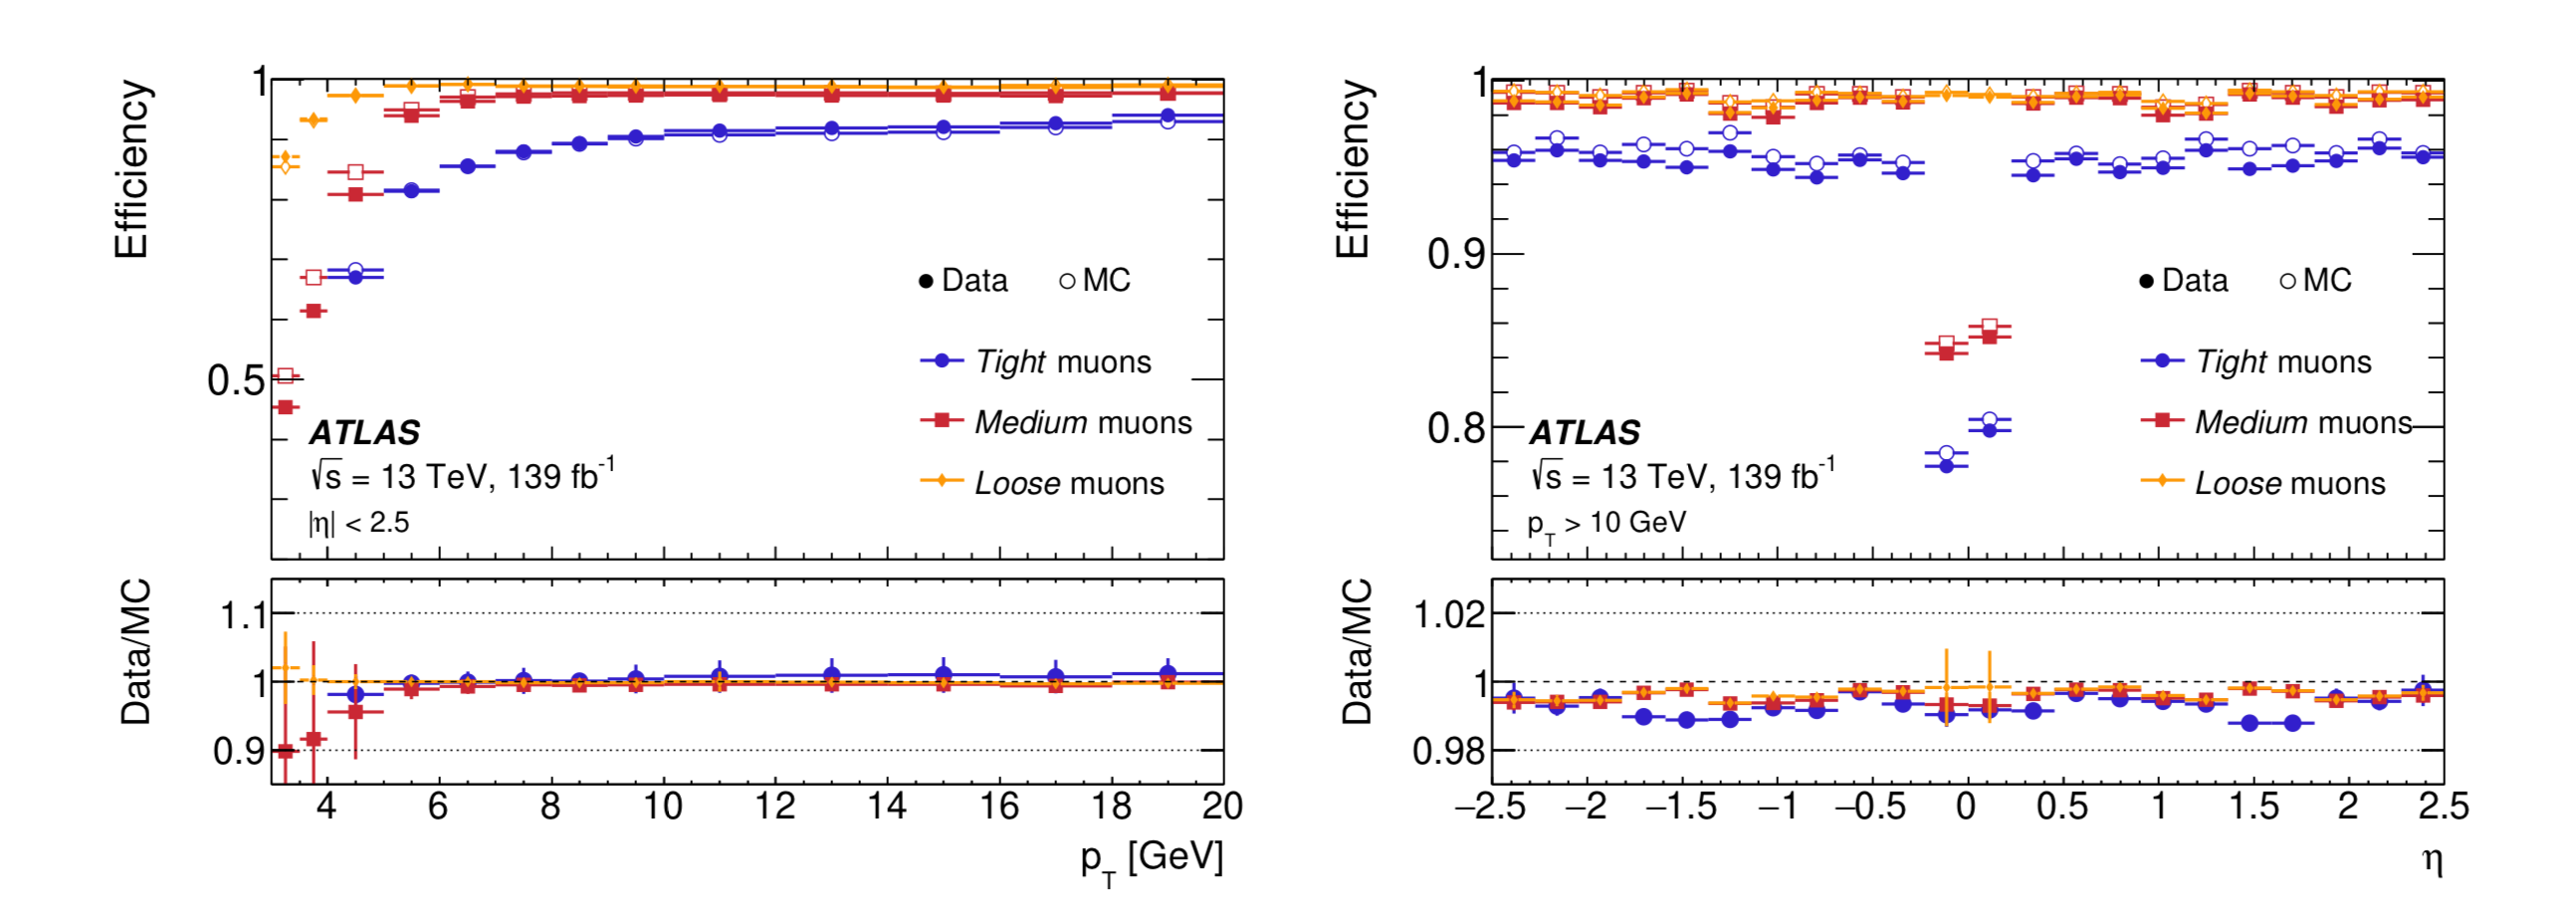
\includegraphics[width=1\textwidth]{figures/common_ana/IdentificationEff}
        \caption{
            This figure shows the reconstruction and identification efficiencies in different variable range in different working points\cite{Aad:2746302}.
        }
        \label{fig:identificationWP}
    \end{center}
\end{figure}



\subsection{Muon Isolation}
Following identification, muon isolation is performed. Other ``non-prompt" muons that resulted from heavy hadron decay before reaching the inner detector. They would not have been cut out from the identification step. Since in comparison, ``prompt muons" usually result in back-to-back isolated higher-$P_{T}$ muons, the relatively high associated neighboring hits from ``non-prompt" heavy flavor muons can be used as criteria for discrimination. The step performed is known as muon isolation. Depending on the muon energy, two different variables are used for muon isolation. One is the track-based isolation and other is calorimeter-based isolation.

\subsubsection*{Isolation Variables}
The parameters used in the isolation criteria are defined as the following:
\begin{itemize}
    \item  $P_{T}^{\textrm{varcone\:size}}$ \newline
        The track-based isolation variable, $P_{T}^{varcone\:size}$ are the sum of the $P_{T}$ of all the tracks in a variable-sized cone. The variable-sized cone(varcone) is defined as below.

    
\begin{equation}
    \delta R = min(\frac{10}{P^{\mu}_{T}[\textrm{GeV}]}, \delta R_{\textrm{varcone\:size}}) 
 \end{equation}

The term is $P_{T}$ dependent, the larger the $P_{T}$, the smaller the cone. 
    \item $E^{\textrm{topocone\:size}}_{T}$ \newline
        A calorimeter based parameter $E^{\textrm{topocone\:size}}_T$ is defined as the sum of the energy deposit in a $\delta R$ size topo cone. 

\end{itemize}
Different working points are developed for balancing ``non-prompt" rejection, ``prompt" acceptance and the isolation performance when in close proximity to other objects. The working points are defined with respect to different variables. Details can be found in~\cite{muon2021}.

\begin{table}[htbp]
\centering
\caption{Definitions of the muon isolation Working points~\cite{muon2021}. }
\begin{adjustbox}{width=1\textwidth}
\begin{tabular}{|c|c|c|}
\hline
Isolation WP & Definition & Track \pT requirement \\
\hline
\emph{PflowLoose}* & $(\ptvarcone[30] +0.4\cdot \pflowiso[20]) < 0.16 \cdot \pT^{\mu}$  & \multirow{2}{*}{$\pT>500$ \MeV} \\
\emph{PflowTight}* & $(\ptvarcone[30] +0.4\cdot \pflowiso[20]) < 0.045 \cdot \pT^{\mu}$ & \\
\hline
\emph{Loose}* & $\ptvarcone[30] < 0.15 \cdot \pT^{\mu}$, $\topoetcone[20] < 0.3 \cdot \pT^{\mu}$  & \multirow{2}{*}{$\pT>1$ \GeV} \\
\emph{Tight}* & $\ptvarcone[30] < 0.04 \cdot \pT^{\mu}$, $\topoetcone[20] < 0.15 \cdot \pT^{\mu}$ & \\
\hline
\emph{HighPtTrackOnly} & $\ptcone[20] < 1.25$ \GeV & \multirow{2}{*}{$\pT>1$ \GeV} \\
\emph{TightTrackOnly}* & $\ptvarcone[30] < 0.06 \cdot \pT^{\mu}$ &  \\
\hline
\multirow{2}{*}{\emph{PLBDTLoose (PLBDTTight)}} & $\ptvarcone[30] < \max(1.8~\GeV,0.15 \cdot \pT^{\mu})$               & \multirow{2}{*}{$\pT>1$ \GeV} \\
& BDT cut to mimic \textit{TightTrackOnly} (\textit{Tight}) efficiency & \\
\hline
\end{tabular}
\label{tab:iso_wp_def}

\end{adjustbox}
\end{table}

%\begin{table}[!htb]
%\begin{tabular}{lllll}
%\begin{adjustbox}{width=1\textwidth}
%\textbf{Isolation Working Point}                                                  & \textbf{Definition} & \textbf{Track PT requirement}   \\ \hline
%\begin{tabular}[c]{@{}l@{}}PFlowLoose\\ PFlowTight\end{tabular}          & $(P_{T}^{\textrm{varcone30}} +0.4 E^{\textrm{netflow20}}_{T}) < 0.16 \cdot P^{\mu}_{T}$ \\ $P_T^{\textrm{varcone30}} + 0.4 E^{\textrm{netflow20}}_{T}) < 0.045 \cdot P^{\mu}_{T} $          &  $P_{T} >500$ MeV                      \\ \hline
%\begin{tabular}[c]{@{}l@{}}Loose\\ Tight\end{tabular}                    & $(P_{T}^{\textrm{varcone30}} < 0.15 \cdot P_{T}^{\mu}, E^{topocone20}_{T}<0.3 \cdot P_{T}^{\mu}$ \\ $(P_{T}^{\textrm{varcone30}} < 0.04 \cdot P_{T}^{\mu}, E^{topocone20}_{T}<0.15 \cdot P_{T}^{\mu}$        &  $P_{T} >$ 1 \\ $P_{T} >$ 1 GeV                      \\ \hline
%\begin{tabular}[c]{@{}l@{}}HighPtTrackOnly\\ TightTrackOnly\end{tabular} &  $P_{T}^{\textrm{cone20}} <$ 1.25 GeV \\ $P_{T}^{varcone30} <0.06 \cdot P_{T}^{\mu}$        &  $P_{T} >1$ GeV                     \\ \hline
%PLBDTLoose (PLBDTTight)                                                  &  $P_{T}^{\textrm{cone30}} < 0.06 \cdot P_{T}^{\mu}$  $(P_{T}^{\textrm{varcone30}} < max(1.8 \textrm{GeV}, 0.15 \cdot P_{T}^{\mu} \\ BDT cut to mimic TightTrackOnly(Tight) efficiency      &  $P_{T} >1$ GeV                    
%\end{tabular}
%\end{adjustbox}
%\end{table}

%The isolation variable cut is often chosen related to the transverse momentum of the muon. For example, in the particle-flow based isolation variable, $P_{T}^{\textrm{varcone 30}}$ is chosen for $P_{T}^{\mu}< 50 GeV and $P_{T}^{\textrm{varcone 30}} is chosen for muons with $P_{T}^{\mu}> 50 GeV$. This provides better efficiency than a single selection. Below in Figure~\ref{fig:isolationWP}.

%\begin{figure}[!htb]
%    \begin{center}
%        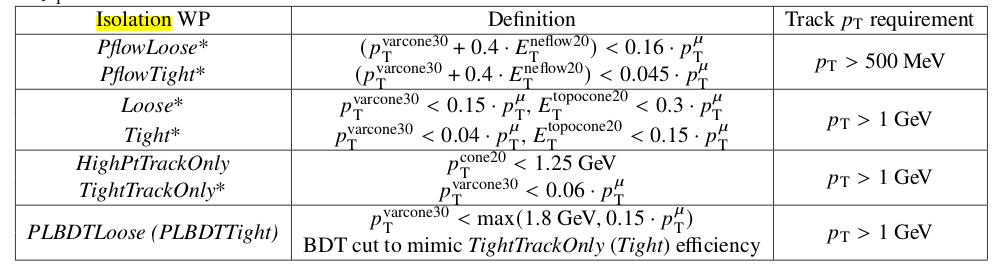
\includegraphics[width=0.75\textwidth]{figures/common_ana/Isolation}
%        \caption 
%        {
%            This figure shows the isolation working points on ATLAS from full run2~\cite{Aad:2746302}.
%        }
%        \label{fig:isolationWP}
%    \end{center}
%\end{figure}

\begin{figure}[!htb]
    \begin{center}
        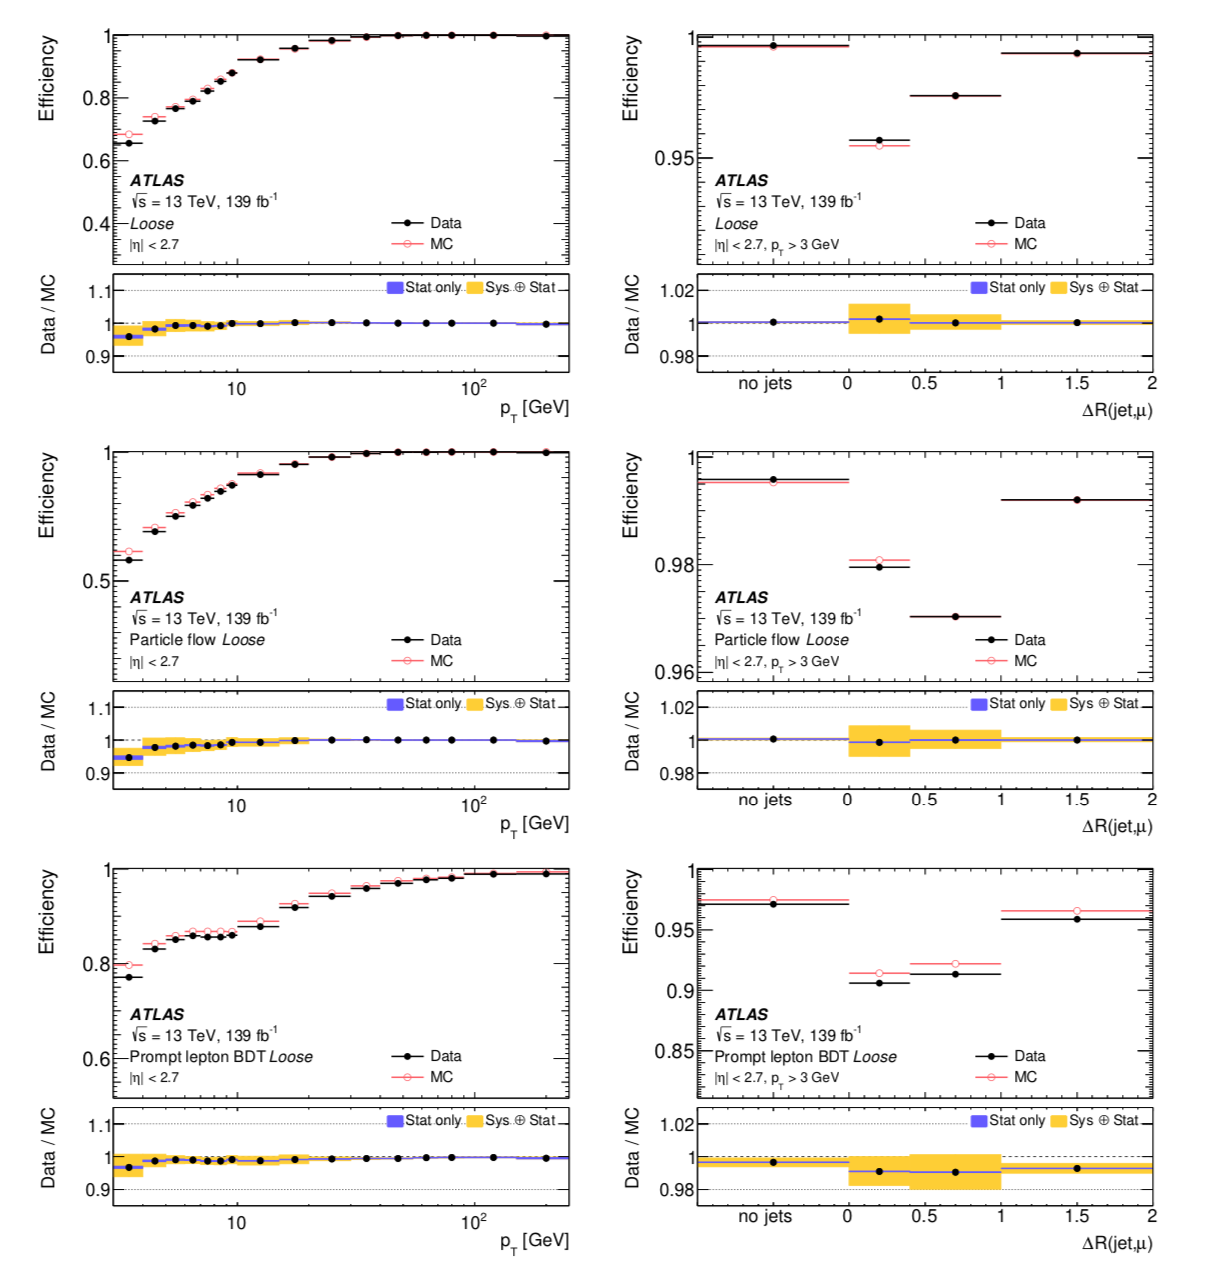
\includegraphics[width=0.75\textwidth]{figures/common_ana/IsolationEff1}
        %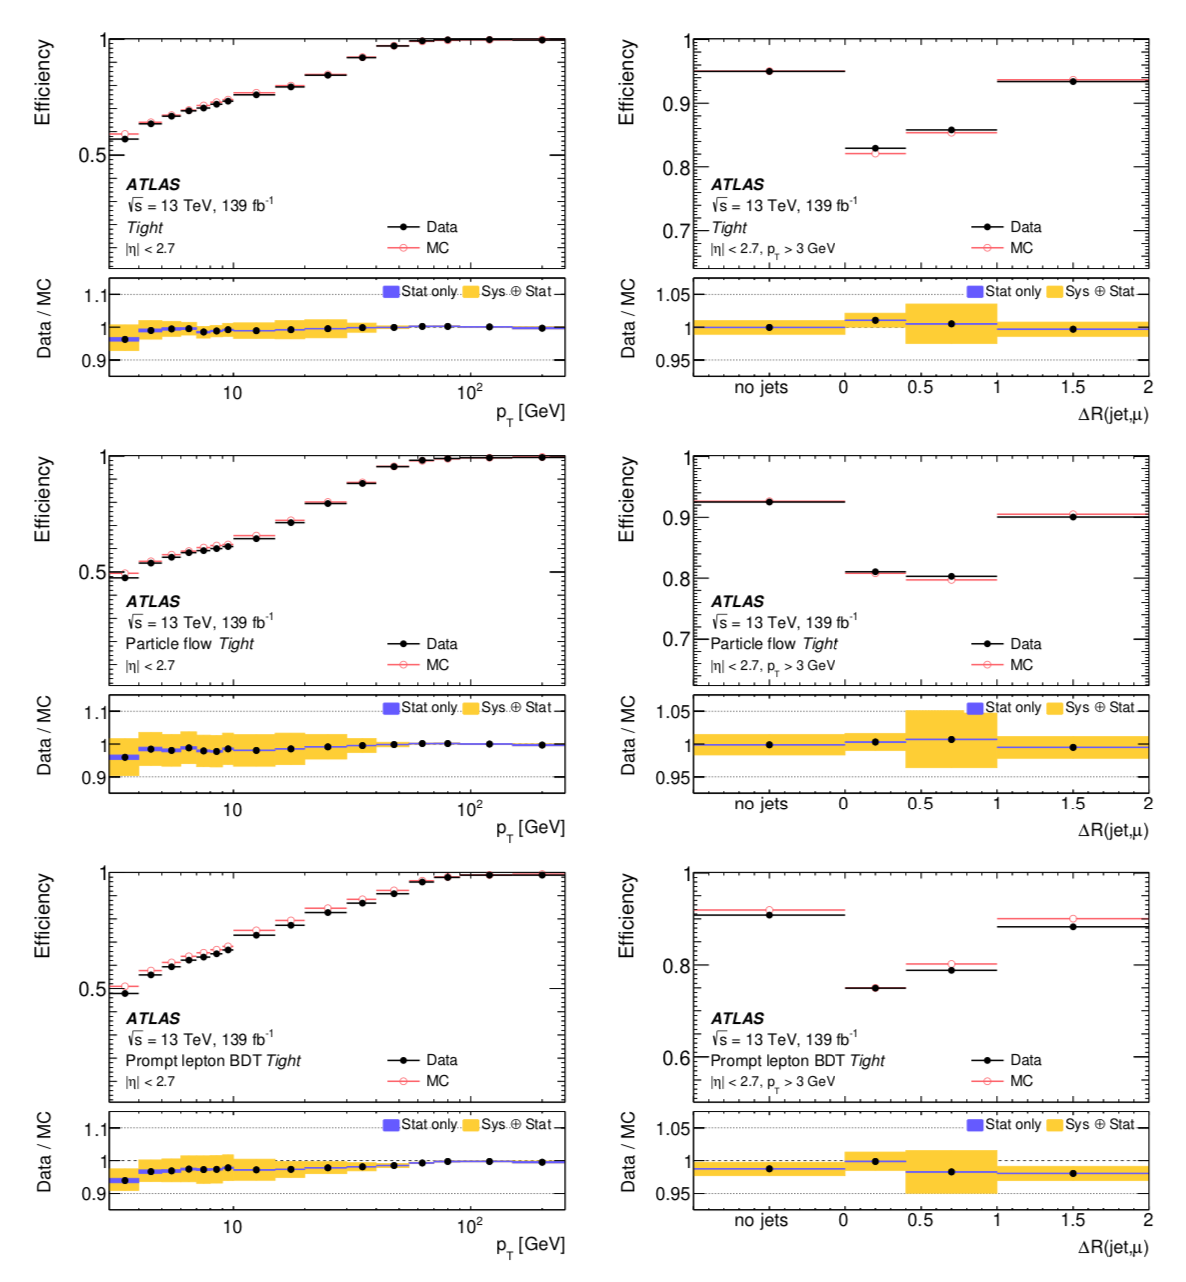
\includegraphics[width=0.75\textwidth]{figures/common_ana/IsolationEff2}
        \caption{
            This figure shows the isolation efficiency in different variable range in different working point\cite{Aad:2746302}.
        }
        \label{fig:isolationWP}
    \end{center}
\end{figure}


\subsection{Muon Calibration}
The Monte Carlo simulation is often imperfect in its parton showering and detector simulation. The imperfection results in difference in data and MC given the same underlying process. This makes understanding the tree level process from the data represent difficult. Given this, a calibration factor is derived from comparing the MC to data using some known physics process $J/\Psi$ to $\mu \mu$ and $Z$ to $\mu \mu$. The calibration is done on the $P_{T}$ of the muon. 
The calibration is dependent on the detector angle, and the formula for $P_{T}$ correction is summarized as below, where the constants are derived from the data and the simulated samples.

%In data there is always margin for calibration error, and monte carlo is also not necessarily accurately describing the experimental environment. To match data result to the actual physics process that happened, transverse momentum correction done on both the MS tracks muons and the ID track on the MC result as follows: 

\begin{equation}
    P_{T}^{\textrm{Cor,Det}} = \frac{P^{\textrm{MC, Det}}_{T} + \sum_{n=0}^{1} S_{n}^{\textrm{Det}}{\eta, \phi}(P_{T}^\textrm{{MC, Det}})^n}{1+\sum_{m=0}^{2}\delta r_{m}^{\textrm{Det}}(\eta, \phi)(P_{T}^({\textrm{MC, Det}})^{(m-1)} g_{m}}
\label{eq:muoncalib}
\end{equation}

Here $P_{T}^{\textrm{MC, Det}}$ is the uncorrected transverse momentum, $g_m$ is a unit Gausssian distribution, $\delta r^{\textrm{Det}}_{m}(\eta, \phi)$ and $S_{n}^{\textrm{Det}}(\eta, \phi)$ are the momentum resolution smearing and scale correction resolution. Det in the equation is short for "Detector, which could be ID or MS. The $S^{Det}_{1}$ term corrects for inaccuraty in the description of the magnetic field, whereas the $S^{Det}_{0}$ corrects for the inaccuracy in the simulation of energy loss in the calorimeter.

The correction is then applied to the combined muon in the following way:

\begin{equation}
    P_{T}^{\textrm{Cor, CB}} = f \cdot P_{T}^{\textrm{Cor, ID}}+ (1-f) \cdot P_{T}^{\textrm{Cor, MS}}
\label{eq:muoncalibfactor}
\end{equation}

The weight f in the above is obtained from MC simulation. $P_T^{\textrm{Cor, CB}}$ and $P_T^{\textrm{Cor,ID}}$ are the corrected transverse momentum in CB and MS respectively.


%\begin{equation}
%\[\delta R = min( \frac{10}/P_{T}[GeV] , \delta R_{max} )\]
%\end{equation}



%For better discrimination effciency, in Run II, ATLAS has moved away from an iterative based method and moved towards a image algorithm for primary vertex finding. A brief description is as the
%following:  
%
%1. A three-dimensional binned box is first defined, the x and y dimension is 4 mm long and the z dimension is 400 mm, a 3-d histogram is made for this 3d box as input data. 
%
%2. Helical tracks are back-projected back to this histogram using a voxel ray-tracking algorithm. All the histogram in each bin crossed by a track is incremented by the path length of the linearized rack in that bin. an example back projected in shown 
%% Whats a vortex ray-tracing algorithm? 
%
%3. This projection is Fourier transformed into frequency sapce.
%
%4. A filter composed of both the angular accpetance of the ATLAS tracking detector in the fourier inverse of the angular acceptance and a four-term Blackman-Harris window filter is used to lessen the effect of high frequency variation is used to multiplied by the projection in the above step. 
%
%5. The filtered image is then transformed back to position space in x, y and z.  
%
%5. The resulting imag is passed to a clustering algorithm where the seeds are identified from the peaks. 

\section{Jets}
\label{sec:Jet}
Colored charge particles interact under the strong force. This includes quarks and gluons. Under the strong force, the energy potential of these color charges increases with their distance apart from each other. The increased potential leads to extra quark and gluon formation as energy and mass is one and the same. This effect is known as parton showering. The color confinement of the strong force result in further hadronization of the showered products.
Showering lead to a cascade of energy deposits in the detector. The jet algorithms aims to reverse the process, it reconstructs the physics properties of the the original primary quark/gluon from the resulting energy deposits. Figure~\ref{fig:jetEvent} is a visualization of an ATLAS event with two high $p_{T}$ jets.

The following is a schematic understanding of how jet finding is achieved. 

$\bullet$ \textbf{Jet showering}

Quark/gluon formed $\rightarrow$  Parton Showering $\rightarrow$ Hadronization $\rightarrow$ Detector Energy Deposit

$\bullet$ \textbf{Jet Reconstruction}

Energy Deposit on Detector  $\rightarrow$  Topo-cell Clustering $\rightarrow$  Topo-Clusters $\rightarrow$  Jet-Finding Algorithm $\rightarrow$ Jet


\begin{figure}[!htb]
    \begin{center}
        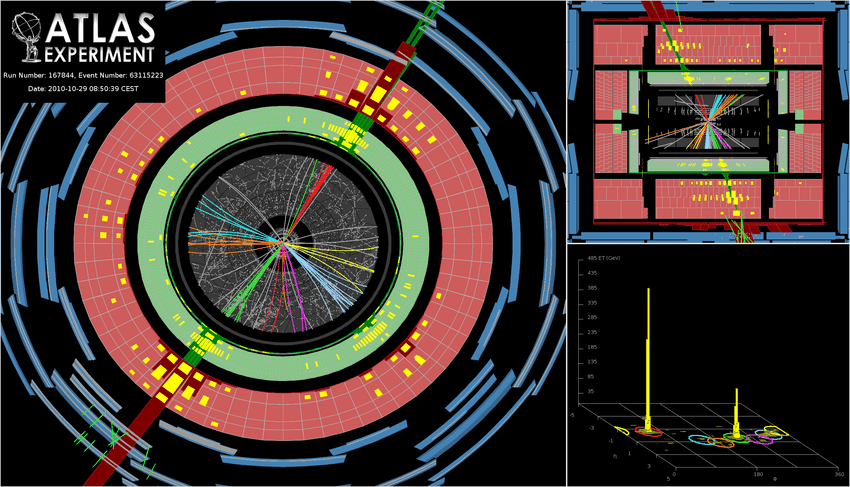
\includegraphics[width=0.7\textwidth]{figures/common_ana/JetEvent}
        \caption{        
            An simulation ATLAS event containing two high $p_{T}$ jet event~\cite{jetEvent}.
        }
        \label{fig:jetEvent}
    \end{center}
\end{figure}

% Why is there a topocell clustering algorithm before jet finding? Maybe it's due to the physics, each one looks like a potential quark/gluon candidate. 
% 
\subsection*{Topo-cell clustering}
\label{Topocell clustering}
This step clusters the lowest level calorimeter cells energy deposits into ``topological clusters", which are cluster of cell deposit with high signal-to-noise (S/N) ratio collected from proximity in the detector. ATLAS uses a 3-D clustering algorithm and it is described as the foolowing:

First, a seed cell with a high S/N ratio above a 4 is found. Then, cells neighboring the seed cells in the in 3 dimensions above S/N 2 are collected along with the seed cell to the topocluster. Lastly, a final set of cells that surround the second set of collected cells above S/N 0  are added to the cluster. 

\subsection*{Jet Finding algorithm}
\label{sec:JetFinding}
% Add the C/A clustering algorithm
% Add the KT algorithm

Jet finding algorithm aims to identify all the deposits that can be traced back to the original hadronic particle. An important feature for a jet finding algorithm is that it needs to be infra-red and collinear(IRC) safe. In an IRC safe algorithm, soft and small angle radiation that showers from the jet will not change the kinematics of the jet. This requirement avoids the divergence in probability calculations that would lead to infinities when jet splitting happens.

All of the main ATLAS jet finding algorithms make use of the following quantities:

\begin{equation}
    d_{ij} = min(k_{ti}^{2p}, k_{tj}^{2p}) \frac{\Delta_{ij}^{2}}{R^{2}}
    \label{sec:topo}
\end{equation}

\begin{equation}
    d_{iB} = k^{2p}_{ti}
\end{equation}

Here, B is the beam, R is the angular distance, $\Delta_{ij}^{2} = (y_{i}- y_{j})^2 + (\phi_{i} - \phi_{j})$, $k_{ti}
$, $y_{i}$, and $\phi_{i}$ are the transverse momentum, rapidity and azimuth angle of particle i. p is a parameter on the energy scale~\cite{HEP2008}. $d_{ij}$ and $d_{iB}$ are the distance between particle i and j and distance between i and B respectively. 

The algorithm clusters the topoclusters with the smallest distance together~\ref{sec:topo}, until no topoclusters are left. p is taken to be -1 for the anti-KT jet finding algorithm; 1 for the KT algorithm and 0 for C/A(in addition, in C/A, $d_{iB} =1$). The Anti-KT algorithm chooses to merge high transverse momentum objects with one another, and the KT algorithm merges low transverse momentum with one another. The C/A algorithm only weights on distance.

The current ATLAS standard jet finding algorithm is the Anti-KT algorithm. It is  an IRC safe algorithm. The algorithm is also not susceptible to underlying events and pile-up as the other two. 

\subsection{Jet calibration} 

After jets are formed, they need to be calibrated to reflect the direction, momentum and energy of the originated quarks or gluons. The jets are required to be calibrated. In ATLAS, jets energy is measured out in both the EM calorimeter and the hadronic calorimeter. The jet finding algorithm operates in the EM scale(as distance in the strong force is energy scale dependent). Jet energy correction needs to be performed before the object can be used for analysis to remove pile up and correct for direction. The jet calibration takes the following steps as shown in Figure~\ref{fig:JetCalibration}.

\begin{figure}[!htb]
    \begin{center}
        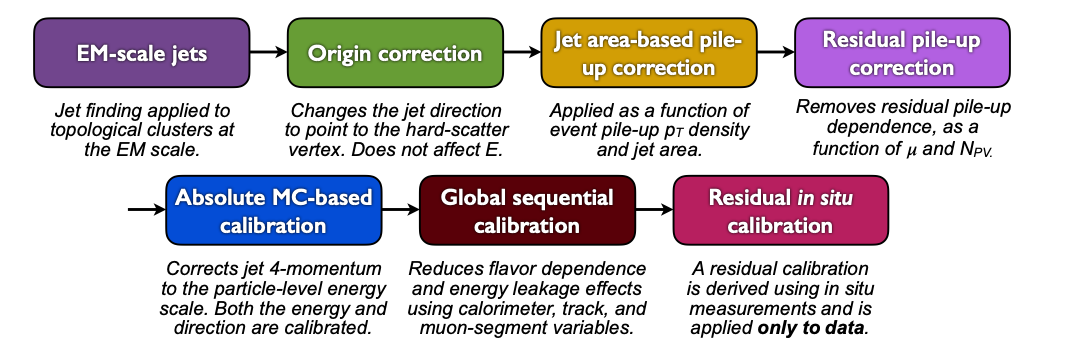
\includegraphics[width=1.1\textwidth]{figures/common_ana/JetCalibration}
        \caption{        
            The steps of calibration performed on the jet objects.\cite{Mehlhase:2770815}. The Jet area is the area of the jet in angular distance for pile-up correction, $\mu$ is the interaction rate per bunchcross and $N_PV$ is the number of primary vertices. The paritcle level scale is the measurement obtained with both the tracker and the calorimeter, energy leakage is the out of cone deposit in the detector that belongs to the original quark/gluon.
        }
        \label{fig:JetCalibration}
    \end{center}
\end{figure}

\section{Photon}
\label{sec:Photon}
Photons in ATLAS are reconstructed from clusters in the EM Calorimeter sometimes paired with tracks in the tracker. Photons and electrons shares a similar reconstruction algorithm. Like muons and jets, photons are first reconstructed, identified, isolated and lastly calibrated before being used for analysis. 

\begin{figure}[!htb]
    \begin{center}
        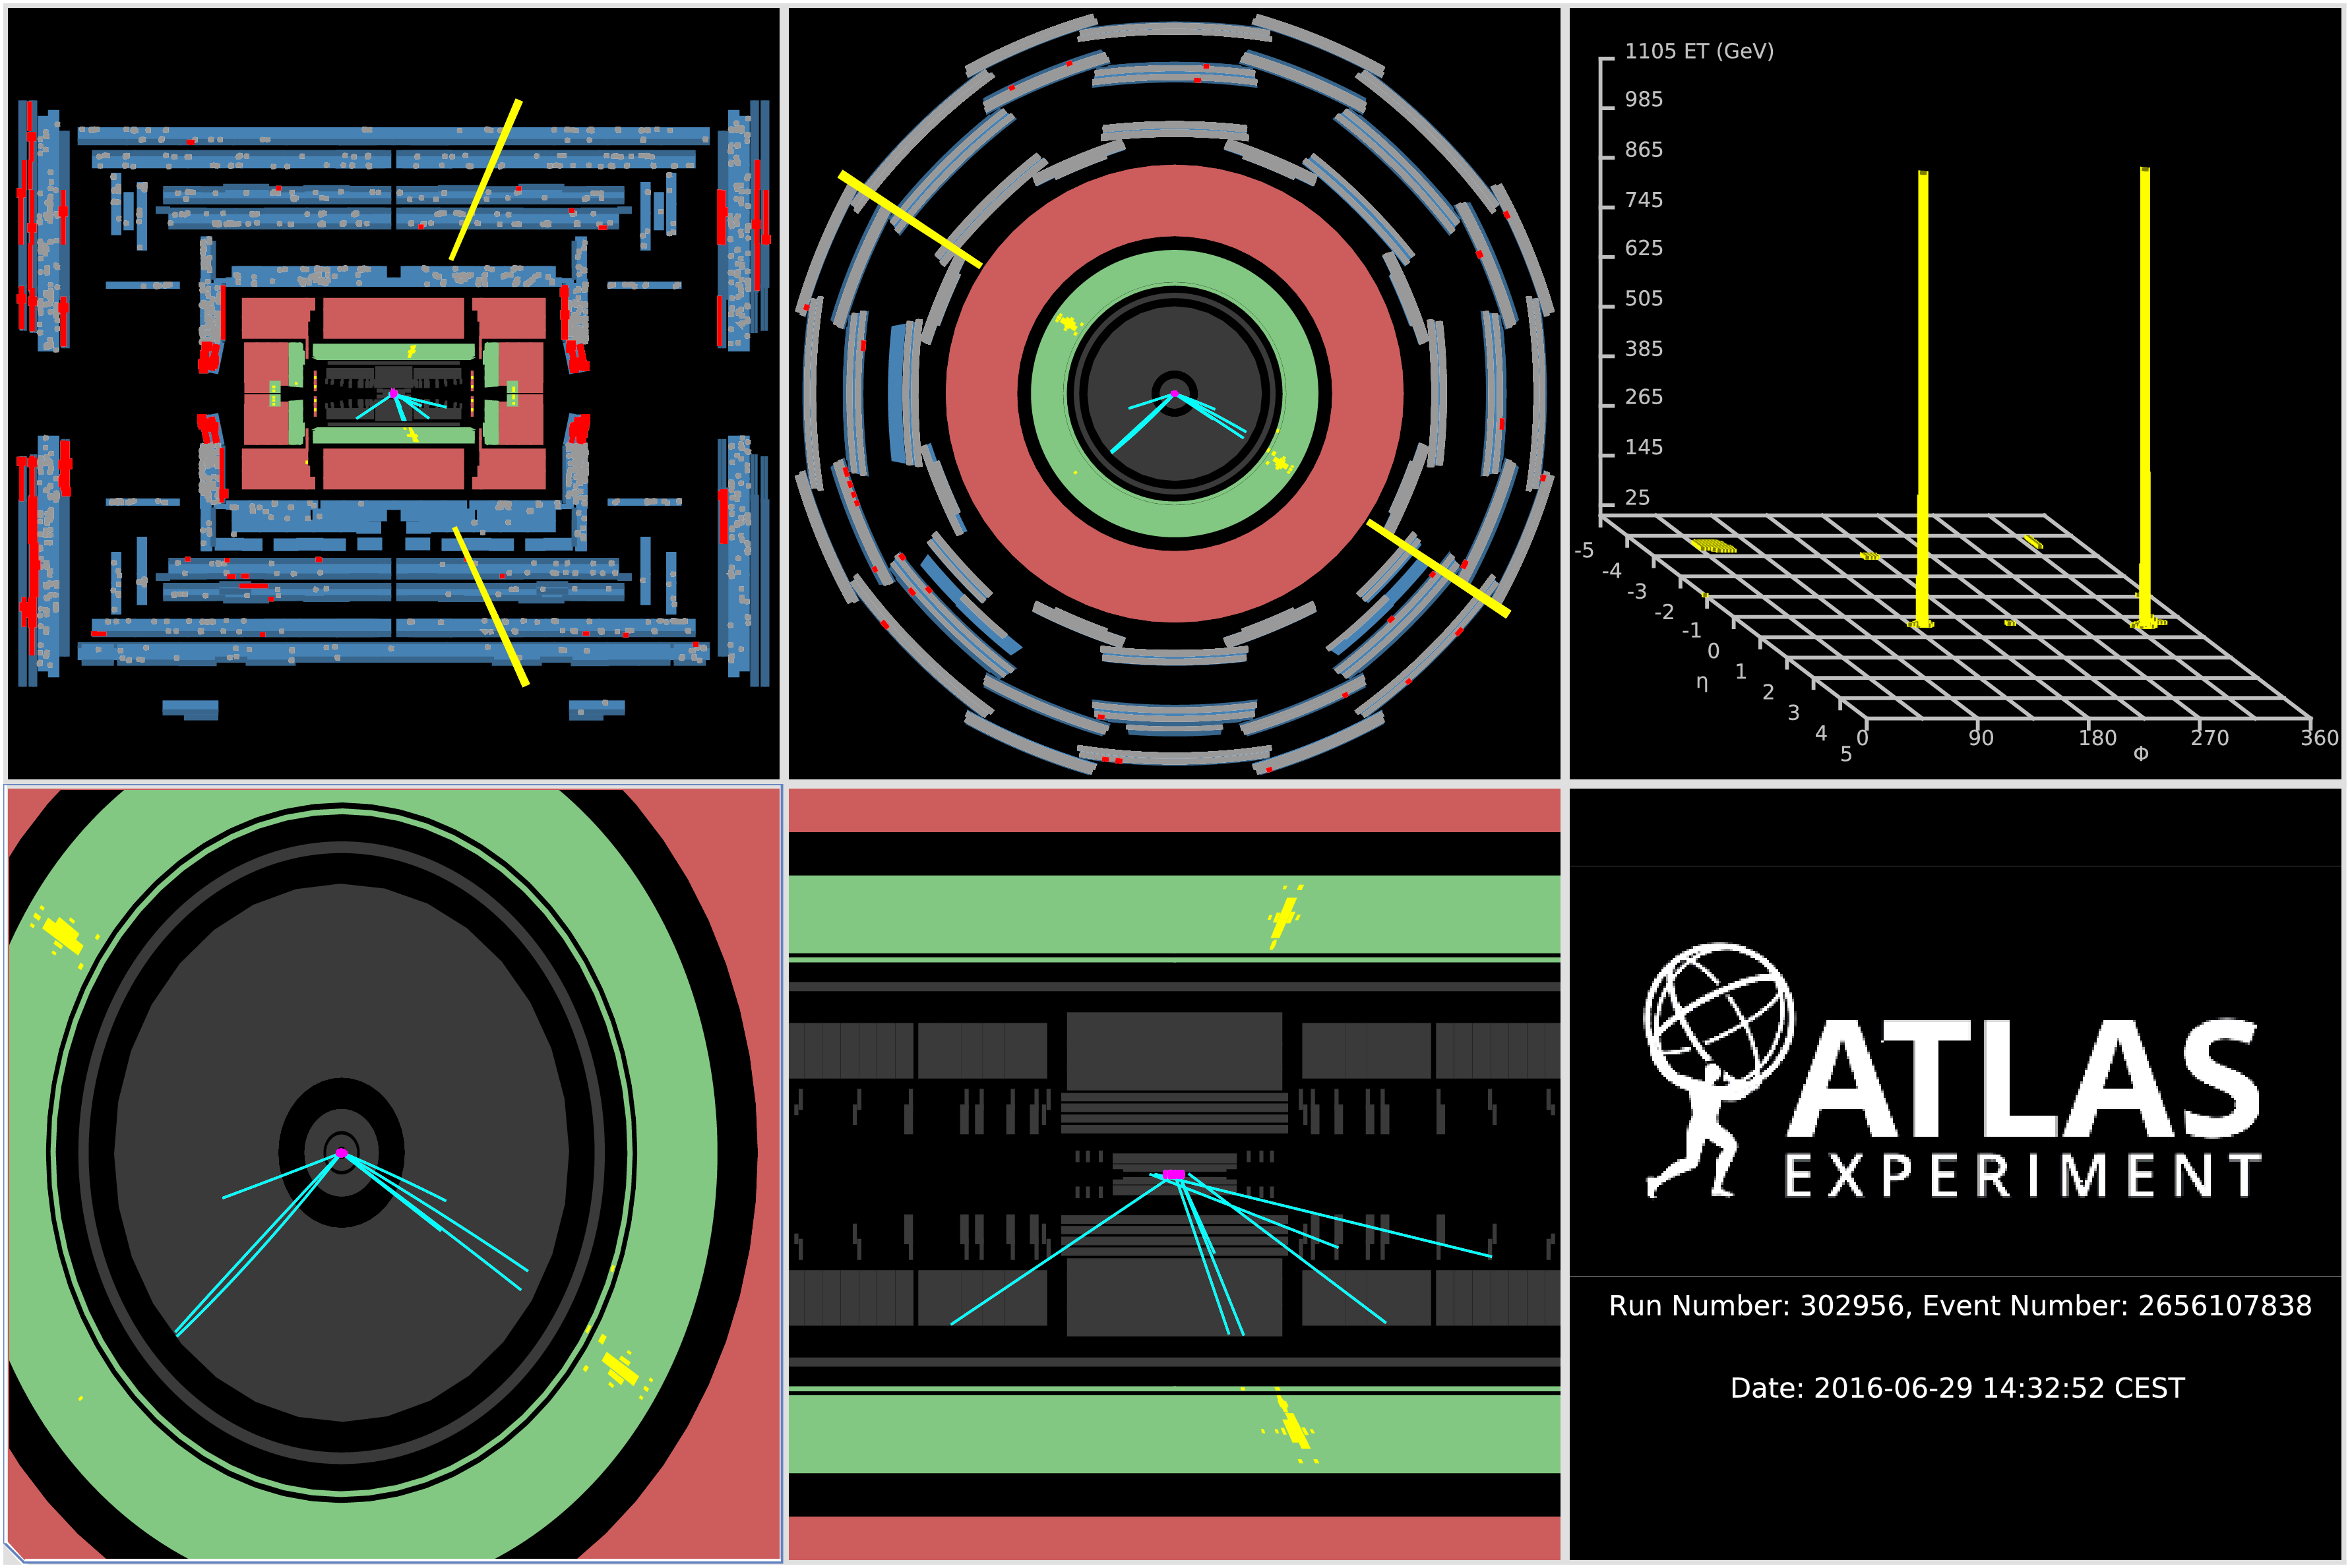
\includegraphics[width=0.7\textwidth]{figures/common_ana/photonEvent}
        \caption{        
        An ATLAS event display that contain two photons~\cite{atlastwophoton}.
        }
        \label{fig:photonEvent}
    \end{center}
\end{figure}

\subsection{Photon Reconstructionn}
Photons interact with the EM calorimeter. They shower and leave deposits in the active material. The first step to photon reconstruction is the finding of a seed cell for clustering. A sliding window of $\delta \eta \times \delta \phi = 0.025 \times 0.0245$ is used to scan for a clustering seed with energy deposit above 2.5 GeV. Neighboring hits are added to the seed to form a cluster through the clustering algorithm~\cite{Lampl:1099735}. 
These cluster are matched by tracks in the inner detector. These tracks are used for vertex construction. If no vertex or tracks are matched, they are unconverted photons, otherwise, they are considered converted photons. Converted photons are photons that originates from electrons. 

%\begin{figure}[!htb]
%    \begin{center}
%        \includegraphics[width=1.1\textwidth]{figures/common_ana/MuonReconstruction}
%        \caption{        
%            Schematics showing the window used to scan the EM Calorimeter for clustering seeds~\cite{gammaCalibration2019}.
%        }
%        \label{fig:MuonReconstruction}
%    \end{center}
%\end{figure}

\subsection{Photon Identification}
Like muons, not all photons candidates are photons generated from the primary vertex. ``Prompt" photons, that came the primary process are of interest in the analysis (dijetISR) worked on. A main source of``non-prompt" photons on ATLAS came from jets decay. Photon identification are mainly placed on shower shapes in the calorimeters~\cite{gammaCalibration2019}.

There are two photon working points, the loose working point uses information from the the calorimeter. The tight working point uses information from the calorimeter strips and has different requirements for uncoverted and converted photon for optimal classfication power. Details can be found in~\cite{gammaCalibration2019}. 

\subsection{Photon Isolation}
Photon isolation is a strategy that is effective in identifying the prompt photons from the ``non-prompt" photons that are produced along other objects. The isolation is a cut on the energy or transverse momentum in $\delta R $ cone size around the photon candidate. The isolation variable for the calorimeter and tracker are calculated separately~\cite{gammaCalibration2019}.

%\begin{itemize}
%
%\item LOOSE \newline
%\begin{equation}
%    E_{T}^{iso}|_{\Delta R < 0.2} < 0.065 \times E_{T}
%\end{equation}
%and 
%\begin{equation}
%    p_{T}^{iso}|_{\Delta R<0.2}<0.05\times E_{T}
%\end{equation}
%
%\item TIGHT \newline
%\begin{equation}
%    E_{T}^{iso}|_{\Delta R<0.4} <0.022 \times 0.022+ 2.45 GeV
%\end{equation}
%and 
%\begin{equation}
%    p_{T}^{iso}|_{\Delta R<0.2 }< 0.05 \times E_{T}
%\end{equation}

%\end{itemize}

\subsection{Photon Calibration}
Photons in ATLAS takes the following steps to be calibrated to correct the estimation of energy deposited in the calorimeter, to correct for the relative energy scale in the different layers of the EM calorimeter, correct for the non-uniformities in the calorimeter response affecting the data and to provide an overall adjustment~\cite{gammaCalibration2019}.
First, the photon energy is estimated from the deposits in the calorimeter by a multivariate regression algorithm trained on simulated events on data. Later, correction is then done on the energy scale in the different layers of the EM calorimeter from Higgs to $\mu \mu$ data, the correction on the calorimeter layers are then applied to the photons calibrated. After that, geometric correction is done on the data to correct for the non-uniformity in the detector in the boundaries of the calorimeter modules. Lastly, an overall adjustment on the energy scale is done in the data~\cite{gammaCalibration2019}.

